\section{Motivation}
\label{sec:methodology}

\subsection{Coherence Traffic}

Our goal in this project, hence is to reduce coherence traffic and coherence misses. As the first step, we did a study on PARSEC benchmark suite to measure coherence traffic. We used Gem5 full-system simulator \cite{GEM5} for this study. Gem5 is a modular event-driven full-system simulator which supports various instruction set architecture such as x86, ARM, Alpha, MIPS and PowerPC.
We used x86 64-bit architecture for our evaluation mainly because this is the only architecture in Gem5 that fully supports various directory coherence protocols. The DRAM simulator is the 
DRAMSim which comes with Gem5 and provides both timing model and power model of DRAM.
As for the operating system, we used Ubuntu 11.04 along with version 2.6.32.3 of the Linux kernel.

  We used the Ruby memory model to monitor coherence traffic. Ruby implements a detailed model for the memory subsystem and enables modeling sophisticated cache coherence protocols. Our system configuration for this study is illustrated in Table \ref{table:sim_param}. The interconnection network is a crossbar which means that each controller (L1/L2/Directory) is connected to every other controller via one switch. Packets, floating through network, are categorized as data or control packets. The control packet is 8 bytes and it includes control messages such as invalidations and write-back acks. The data packet is 64 bytes and it carries the data. We measure the traffic by monitoring packets flowing through each controller.\\

\begin{table}
  \centering
  \begin{tabular}{||c|c||}
	\hline
	\multicolumn{2}{||c||}{\textbf{Processor}}\\
	\hline
	ISA & x86-64 \\ \hline 
	CMP size and Core Freq. & 4-core, OoO, 2 GHz \\ \hline
	Re-order Buffer & 128 entry \\ \hline
	
	\multicolumn{2}{||c||}{\textbf{Cache Hierarchy}} \\
	\hline
	L1 I-cache & 64KB/2-way, 2-cycle \\ \hline
	L1 D-cache & 64KB/2-way, 2-cycle \\ \hline
	L2 Cache & 4MB/16-way, shared, 20-cycle \\ \hline
	Coherence Protocol & MESI Directory \\
	\hline

    \multicolumn{2}{||c||}{\textbf{DRAM Parameters}} \\
    \hline
    DRAM device parameters & Micron x8 4Gb chip, 8 chips \\ \hline
	Memory Channel & DDR3 800 MHz channel, 1 channel \\ \hline
	Number of banks & 8 banks/device \\ \hline
  \end{tabular}
  \caption{Simulator Parameter}
  \label{table:sim_param}		

\end{table}

\begin{figure}[h]
  \centering
  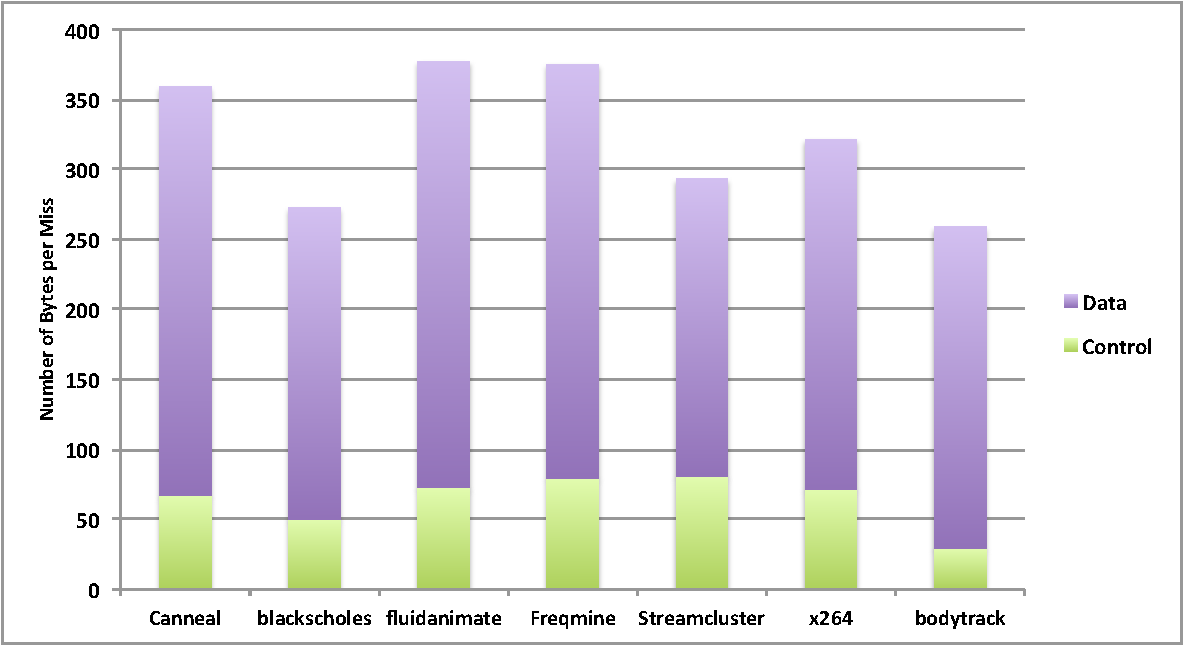
\includegraphics[height=2.2 in, width=3.2in]{figures/Network-traffic.pdf}
  \caption{Number of bytes flowing through network per miss}
  \label{fig:profile}
\end{figure}

Figure 1 presents coherence traffic flowing through L1 cache controller. The y axis indicates the total number of bytes (data and control packets) normalized to the number of L1 cache misses. As it is shown in the figure 1, for most of the benchmarks, around 120 bytes traffic goes through each L1 cache controller per each L1 cache miss, instead of 64 bytes. This additional traffic, which is mainly dominated by data packets, is because of data exchange and coherence messages between threads sharing the same data. Figure 2 shows the coherence traffic across the network which is measured by monitoring packets going through all controllers (L1,L2 and Directory). For most of the benchmarks, the amount of traffic is around 300 bytes per cache miss. Our analysis indicates that when application exhibits high degree of sharing, coherence traffic becomes a major bottleneck, especially by increasing the number of threads.  


\begin{figure}[h]
  \centering
  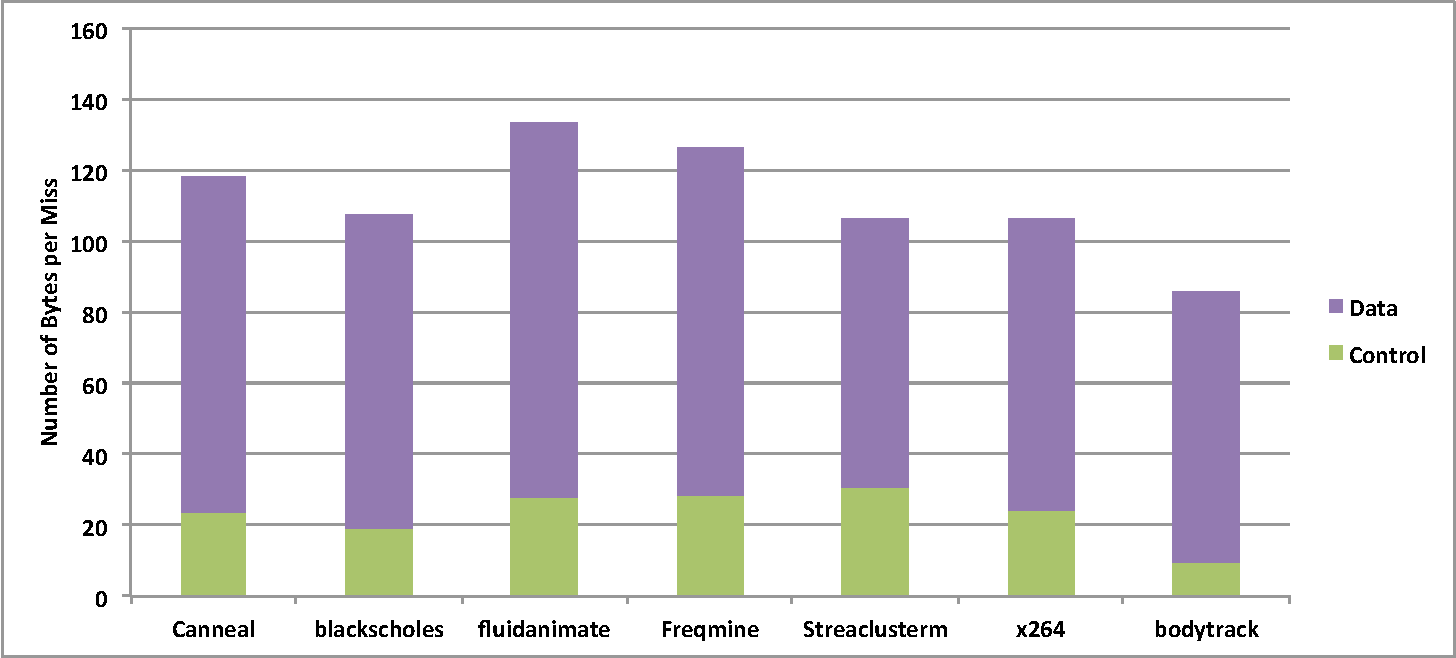
\includegraphics[height = 2.2 in, width=3.4in]{figures/figure1.pdf}
  \caption{The number of bytes flowing through L1 cache per miss.}
  \label{fig:profile}
\end{figure}



\subsection{Approximate Coherence}

Coherence ensures perfect correctness and precision of data. It guarantes that changes in shared data are propagated throughout the system in a timely fashion. The question is that is it always necessary? Is it always required to guarantee perfect correctness? This question leads us to the motivation of our project. If we could somehow tolerate imprecision, we would then be able to trade-off precision to reduce the coherence traffic. The next question would be what applications could tolerate such imprecision? As we mentiond, applications in approximate computing domain could fit well to this purpose. Let's walk through an example to see how we can exploit imprecision of data to reduce coherence traffic. Assume we have four threads, each reading and writing to a shared value, called X. Assume that X could be approximated and the error margin is 20\%. Figure 3 shows a piece of code for such a program. It is assumed that the program is already annotated (data-centric approximtion). Figure 4 shows the cache content during the execution of this code. As it is illustrated in Figure 4a, thread 1 first reads the value X and brings it to its own cache (second line of code). At line 3, thread 1 performs a computation and updates the value of X. The approximated result of computation is 2.1 and the precise value is 2 (It is in the error margin). After that, it updates the value of X in the L1 cache (Figure 4b). The other threads then begin reading value of X (Figure 4c). At line 7, thread 2 executes the function. The approximated result of the function is 2.2 and the precise value is again 2. Thread 2 then wants to update the value of X, and to maintain cache coherence, it is required to obtain exclusive permission and invalidate all other shared copies. However, 2.2 is an approximate value of 2 and it is in the error margin. Since it is an approximated value of 2, both 2.2 and 2.1 could be treated as a same value. As a result, we could simply update thread 2 L1 cache and let other threads keep the previous value of X in their caches (Figure 4d). Such an approach allows us to eliminate 7 control messages (GetX request, Invalidations and Acks) and avoid coherence misses when other threads attempt to access value of X. 

The above example indicates the key motivation behind our idea. Increasing number of thread makes coherence traffic a major bottlneck. It leads to excessive number of invalidations and coherence message, which lead to performance and power efficiency degradation.
  
\begin{figure}[h]
  \centering
  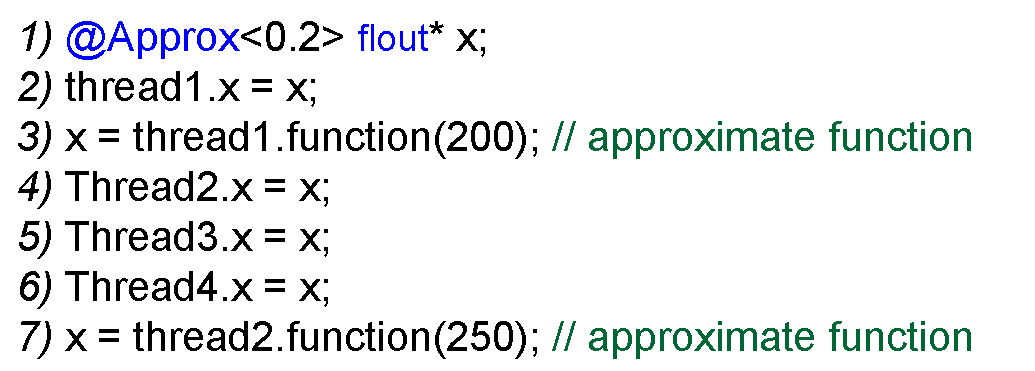
\includegraphics[height=1.2 in, width=3.2in]{figures/figure3.pdf}
  \caption{Pseudo Code}
  \label{fig:profile}
\end{figure}


\begin{figure}[h]
  \centering
  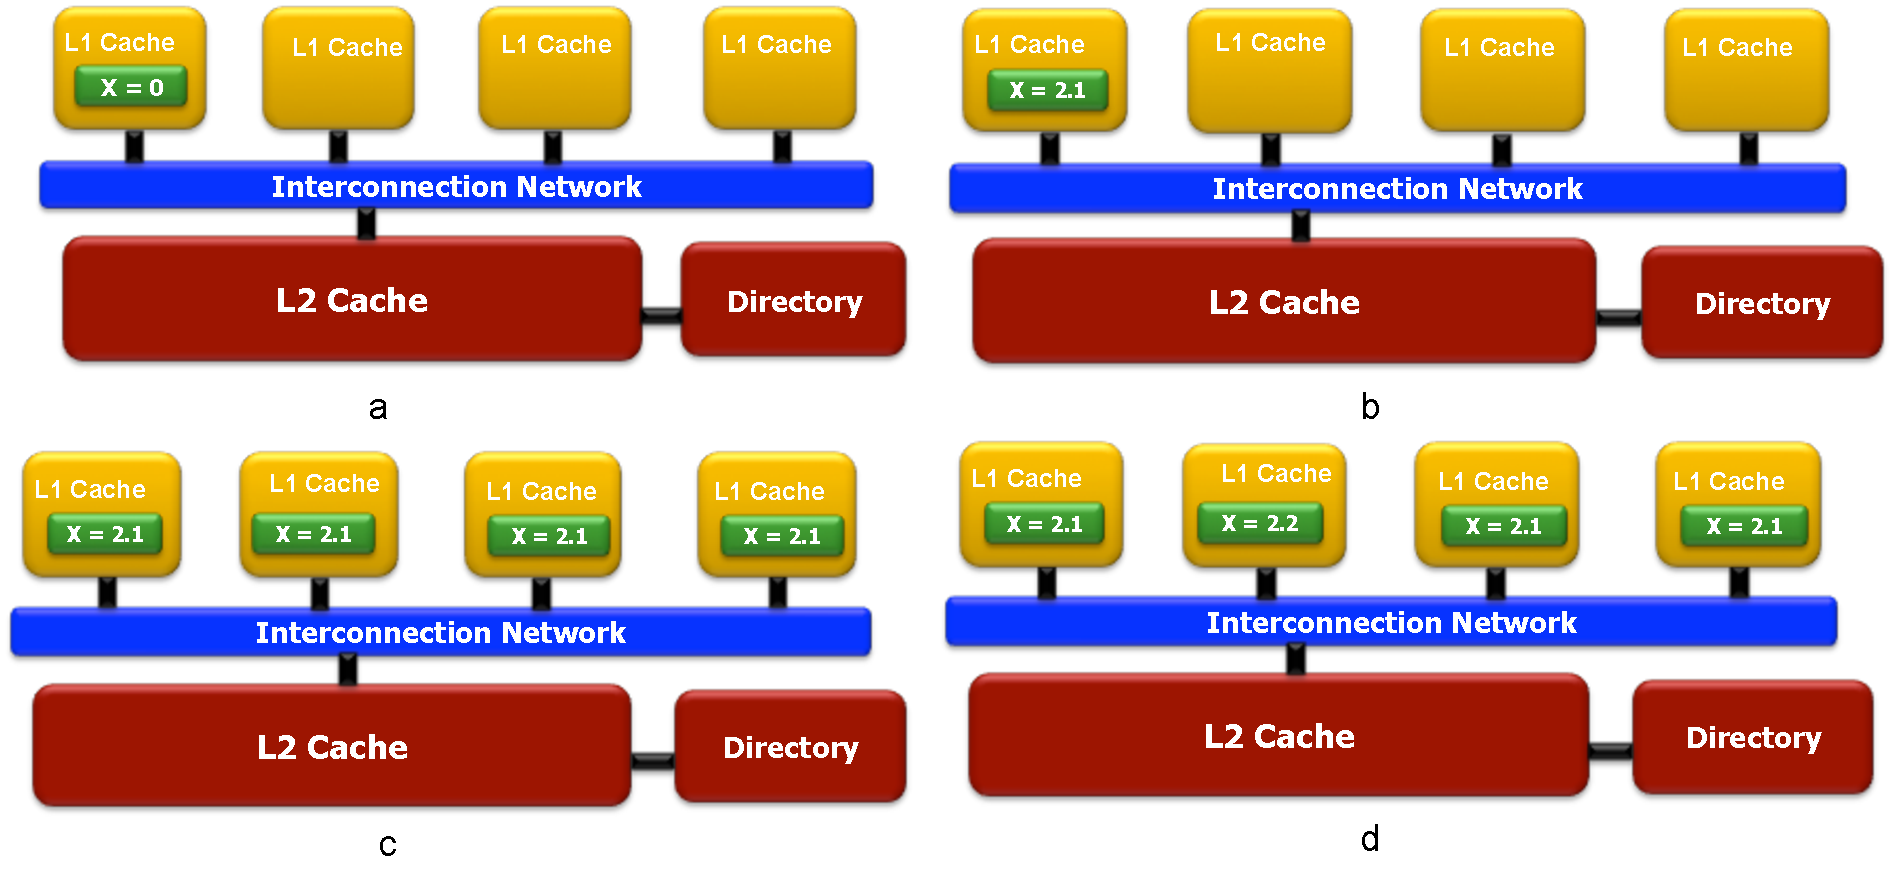
\includegraphics[height = 2.5 in, width=3.5in]{figures/figure4.pdf}
  \caption{Cache content during code execution. (a) Thread 1 reads X (b) Thread 1 does the approximate computation and writes 2.1 to X. The precise value is 2. (c) Other threads read the value of x. (d) Thread 2 writes 2.2 to X. The precise value is again 2.}
  \label{fig:profile}
\end{figure}



